\Chapter{}

% \chapter{CRONOGRAMA DE ACTIVIDADES}
%     \begin{figure}[H] 
%         \caption{\doublespacing \\ \textit{Cronograma de actividades para la investigación.}} 
%         \centering
%         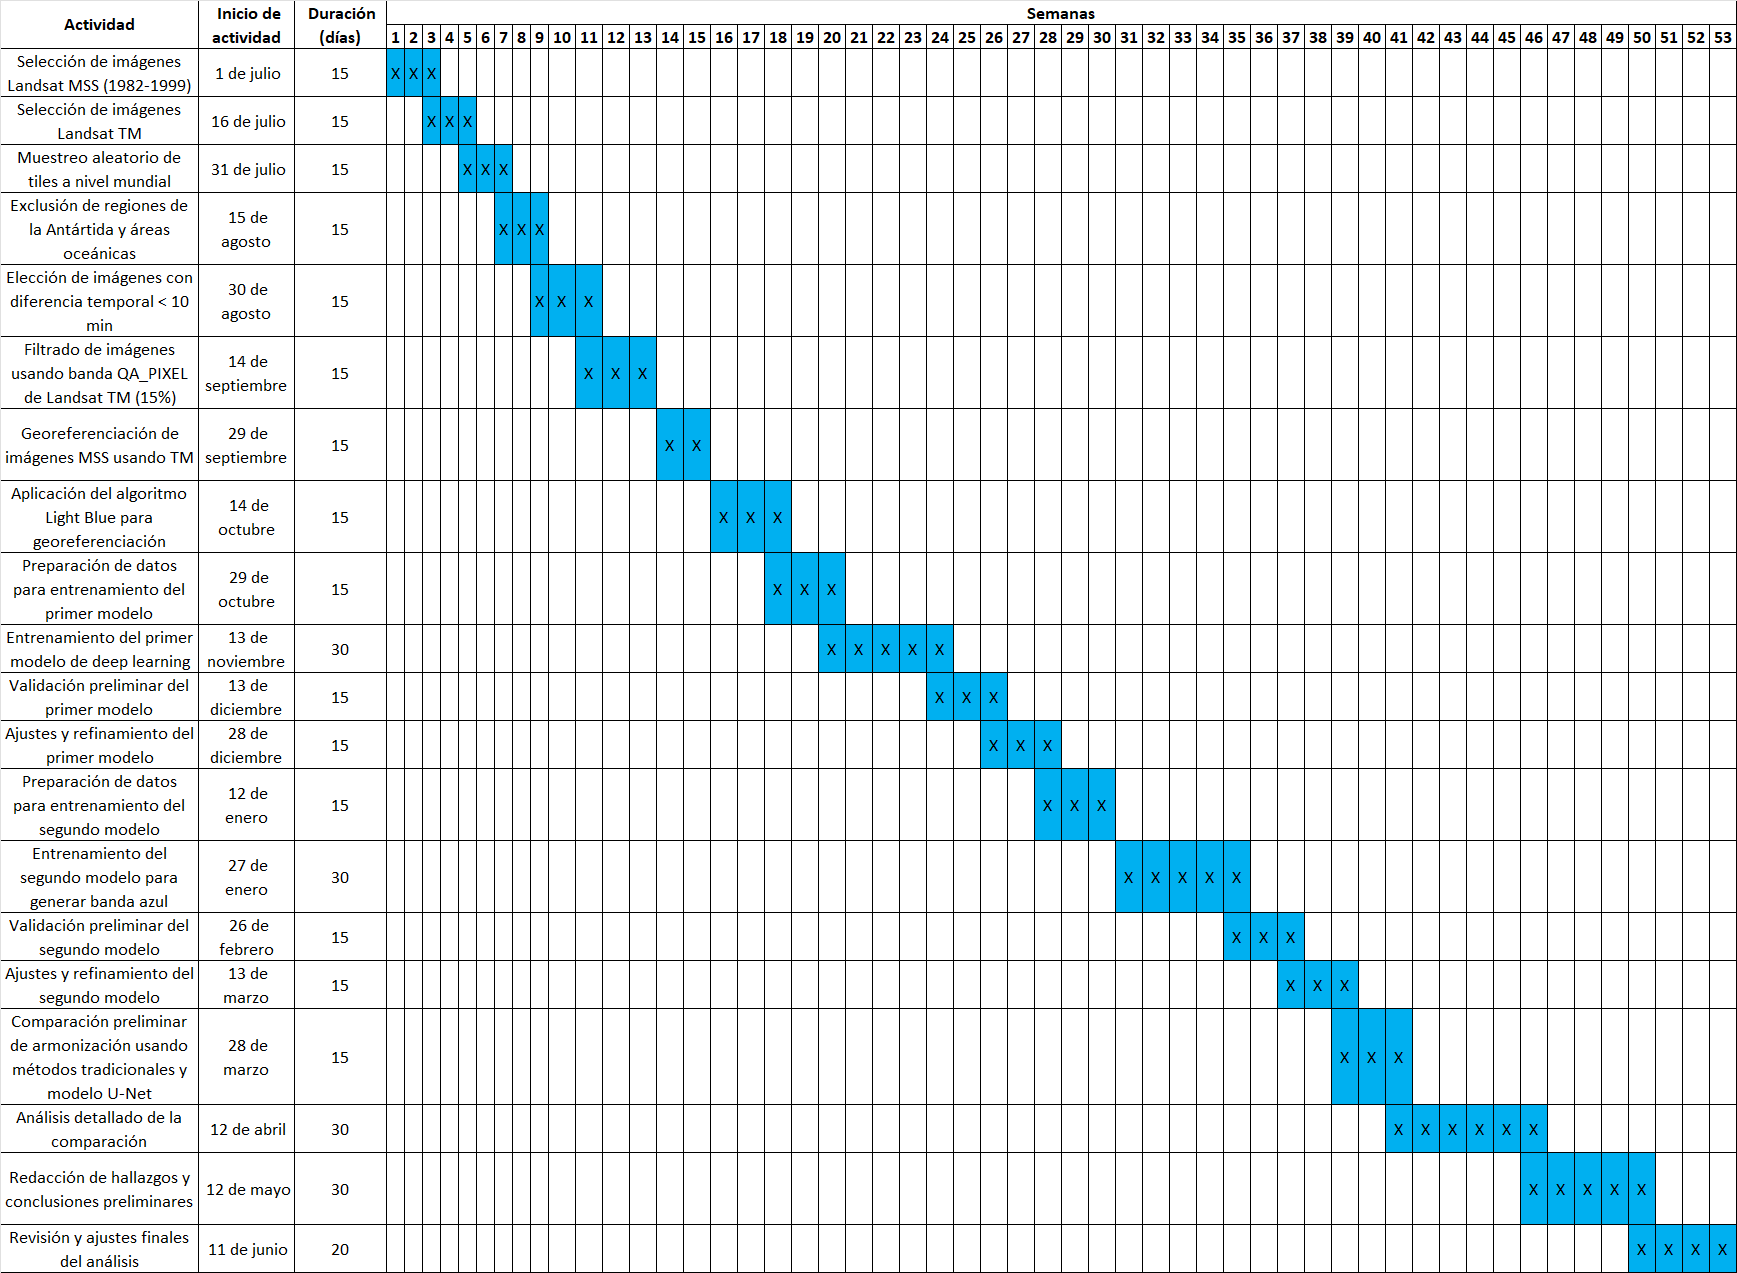
\includegraphics[width=1.12\linewidth, angle=90]{2_CAPITULO0/IMG/cronograma.png}
%         \begin{justify}
%             \textit{Nota.} El cronograma anual detalla la secuencia de actividades, desde la elección de imágenes Landsat hasta las modificaciones finales, organizadas semanalmente a lo largo de un año.
%         \end{justify}                    
%         \label{cronograma}
%     \end{figure}

\chapter{DISCUSIÓN}

    La validación cuantitativa del modelo SWINIR - MSS2TM se centró en la precisión espectral y la superresolución, destacando la selección estratégica de Perú por su diversidad topográfica y ecosistémica. Comparado con estudios previos en el campo, este modelo demostró un rendimiento competitivo y estuvo en línea con los avances más recientes en la literatura científica relacionada con la superresolución y la armonización de imágenes satelitales .

    \section{Evaluación comparativa con estudios previos}
        Los resultados obtenidos indicaron que el modelo SWINIR - MSS2TM no solo mejoró la alineación espacial de las imágenes MSS respecto a las TM, sino que también optimizó la armonización espectral, como lo demostraron las mejoras significativas en los índices espectrales NDVI, NDWI y NDSI. Estos avances fueron comparables, si no superiores, a los logrados en estudios similares recientes, destacando el potencial de las técnicas de aprendizaje profundo en el procesamiento de imágenes satelitales .

    \section{Variabilidad geográfica y rendimiento del modelo}
        A pesar del buen rendimiento general del modelo, evidenciado por las métricas de MAE, RMSE y el coeficiente de Pearson, se observaron variaciones notables en la efectividad de la superresolución entre diferentes regiones geográficas. Específicamente, los resultados subóptimos en la imagen 06008, ubicada sobre el Lago Titicaca, destacaron los desafíos asociados con cuerpos de agua, donde la interferencia atmosférica y la homogeneidad espectral pueden degradar la precisión del modelo. Este fenómeno sugirió que el modelo podría beneficiarse de ajustes o configuraciones específicas cuando se enfrenta a condiciones espectralmente homogéneas o interferencias atmosféricas.

    \section{Implicaciones prácticas y limitaciones}
        Las implicaciones prácticas de los resultados fueron considerablemente positivas, particularmente para aplicaciones que demandan alta fidelidad en la interpretación de datos satelitales. La capacidad del modelo para mejorar la resolución y precisión espectral de las imágenes MSS facilitó aplicaciones en cartografía, gestión de recursos naturales y monitorización ambiental. Sin embargo, las limitaciones observadas en cuerpos de agua y bajo condiciones atmosféricas adversas requirieron un enfoque más especializado. La integración de métodos que pudieran compensar estas condiciones podría mejorar sustancialmente la versatilidad y la eficacia del modelo .

